
\section{App auf Rezept}
Wie bereits erwähnt würde am 19.Dezember 2019 mit der Inkraftsetzung des Digitale-Versorgungs-Gesetzes (DVG), die ``App auf Rezept'' für Patientinnen und Patienten in die Gesundheitsverordnung eingeführt. Digitale Gesundheitsanwendungen (DiGA) können somit von Ärzten und Psychotherapeuten verordnet und durch die Krankenkasse erstattet werden. Dies eröffnet vielfältige Möglichkeiten, um bei der Erkennung und Behandlung von Krankheiten sowie auf dem Weg zu einer selbstbestimmten gesundheitsförderlichen Lebensführung zu unterstützen.

``Das BfArM hat diesen bedeutenden Baustein der Digitalisierungsstrategie der Bundesregierung und des Bundesgesundheitsministeriums von Anfang an mitgestaltet und unterstützt Hersteller und Anwender digitaler Medizinprodukte wie z.B. Medical Apps seit Jahren intensiv u.a. bei Fragen zur Einstufung einer App als Medizinprodukt oder zur Cybersicherheit von Medizinprodukten.'' /cite(https://diga.bfarm.de/de)

``Das Bundesinstitut für Arzneimittel und Medizinprodukte (BfArM) ist eine selbstständige Bundesoberbehörde im Geschäftsbereich des Bundesministeriums für Gesundheit (BMG). [... Es hat in diesem Kontext] die Aufgabe, Anträge zur Aufnahme von DiGA in das Verzeichnis wissenschaftlich zu bewerten. Es stellt außerdem das Verzeichnis für digitale Medizinprodukte bereit, die nach erfolgreicher Prüfung als erstattungsfähige digitale Gesundheitsanwendungen (DiGA) gelistet werden'' /cite(https://diga.bfarm.de/de)

Über sogenannte ``Bekanntmachungen'' im Bundesanzeiger, die erstmals am \textit{06.1.2020}~\cite{https://diga.bfarm.de/assets/documents/201006_BfArM_Bekanntmachung-DiGA-1.pdf} und zuletzt am \textit{29.12.2020}~\cite{https://diga.bfarm.de/assets/documents/201229_BfArM_Bekanntmachung-DiGA-2.pdf} erschienen sind, werden Informationen wie die Errichtung des Verzeichnisses für digitale Gesundheitsanwendungen (DiGA), die Bildung neuer Gruppen oder die Veränderung bestehender Gruppen im DiGA-Verzeichnis, die Aufnahme neuer DiGA im DiGA-Verzeichnis, die Streichung von DiGA aus dem DiGA-Verzeichnis veröffentlicht. Diese Veröffentlichung folgt vierteljährlich.

Für ärztliche oder psychotherapeutische Leistungserbringer eröffnet das Verzeichnis vielfältige Möglichkeiten, sich einen Überblick über verfügbare DiGA zu verschaffen, die möglicherweise für ihre Patienten infrage kommen könnten. Die im Verzeichnis aufgeführten Informationen sollen das gemeinsame aussuchen mit dem Patienten, unterstützen. Sodass die zur aktuellen Situation am besten geeignete DiGA verordnet werden kann.

\subsection{Wie kann eine DiGA verordnet werden?}

(https://diga.bfarm.de/de/leistungserbringer)
Im Verzeichnis finden Sie wichtige Informationen, die Sie unmittelbar zur Verordnung einer von Ihnen ausgewählten Verordnungseinheit (DiGA-VE) der erstattungsfähigen DiGA für einen Patienten mit vorliegender Indikation nutzen können.
Die wesentlichen verordnungsrelevanten Informationen werden, ggfs. mit einem gewissen, technisch bedingten Zeitverzug, auch von Ihrem Praxisverwaltungssystemhersteller unmittelbar in Ihrem Praxisverwaltungssystem (PVS) bereitgestellt.
Schlüssel zur Verordnung einer bestimmten DiGA-VE (z.B. ein bestimmtes DiGA-Modul für einen bestimmten Verordnungszeitraum) ist, analog z.B. zu unterschiedlichen Dosierungen und Packungsgrößen bei Arzneimitteln, die Pharmazentralnummer (PZN), die dazu auf dem Verordnungsvordruck (Muster 16) aufzufinden ist ,anzugeben.
Bitte beachten Sie dazu die Hinweise z.B. der Kassenärztliche Bundesvereinigung (KBV) sowie ggfs. Ihres PVS-Herstellers.
Zu jeder DiGA wird im Verzeichnis auf der Informationsseite für Leistungserbringer u.a. eine Tabelle vorgesehener Verordnungseinheiten einschließlich der jeweiligen Eigenschaften und der zugehörigen PZN angegeben.

Das BfArM ist nicht in den Verordnungs- bzw. Erstattungsprozess für DiGA eingebunden, an dieser Stelle möchten wir nochmal darauf aufmerksam machen, wie dieser Prozess vorgesehen ist und wo Sie weitere Informationen dazu erhalten können.

Nachdem die passende Verordnungseinheit einer DiGA mit der entsprechenden Pharmazentralnummer (PZN) auf einem üblichen Kassenrezept (Muster 16) verordnet wurde, kann der Patient dieses bei seiner gesetzlichen Krankenkasse einreichen und um Zusendung eines Freischaltcodes für die DiGA bitten. Dieser wird ihm dann von der Krankenkasse zugesandt einschließlich weiterer Hinweise, unter welchem Link die DiGA heruntergeladen oder der Hersteller der DiGA dazu kontaktiert werden kann (z.B. falls zusätzliche Hardware Bestandteil der DiGA ist).
Nach der Aktivierung der DiGA unter Nutzung des Freischaltcodes kann die DiGA für den verordneten Zeitraum genutzt werden und der DiGA-Hersteller rechnet die Kosten unter Bezug auf den verwendeten Freischaltcode direkt mit der Krankenkasse ab.

\begin{figure}[H]
	\centering
	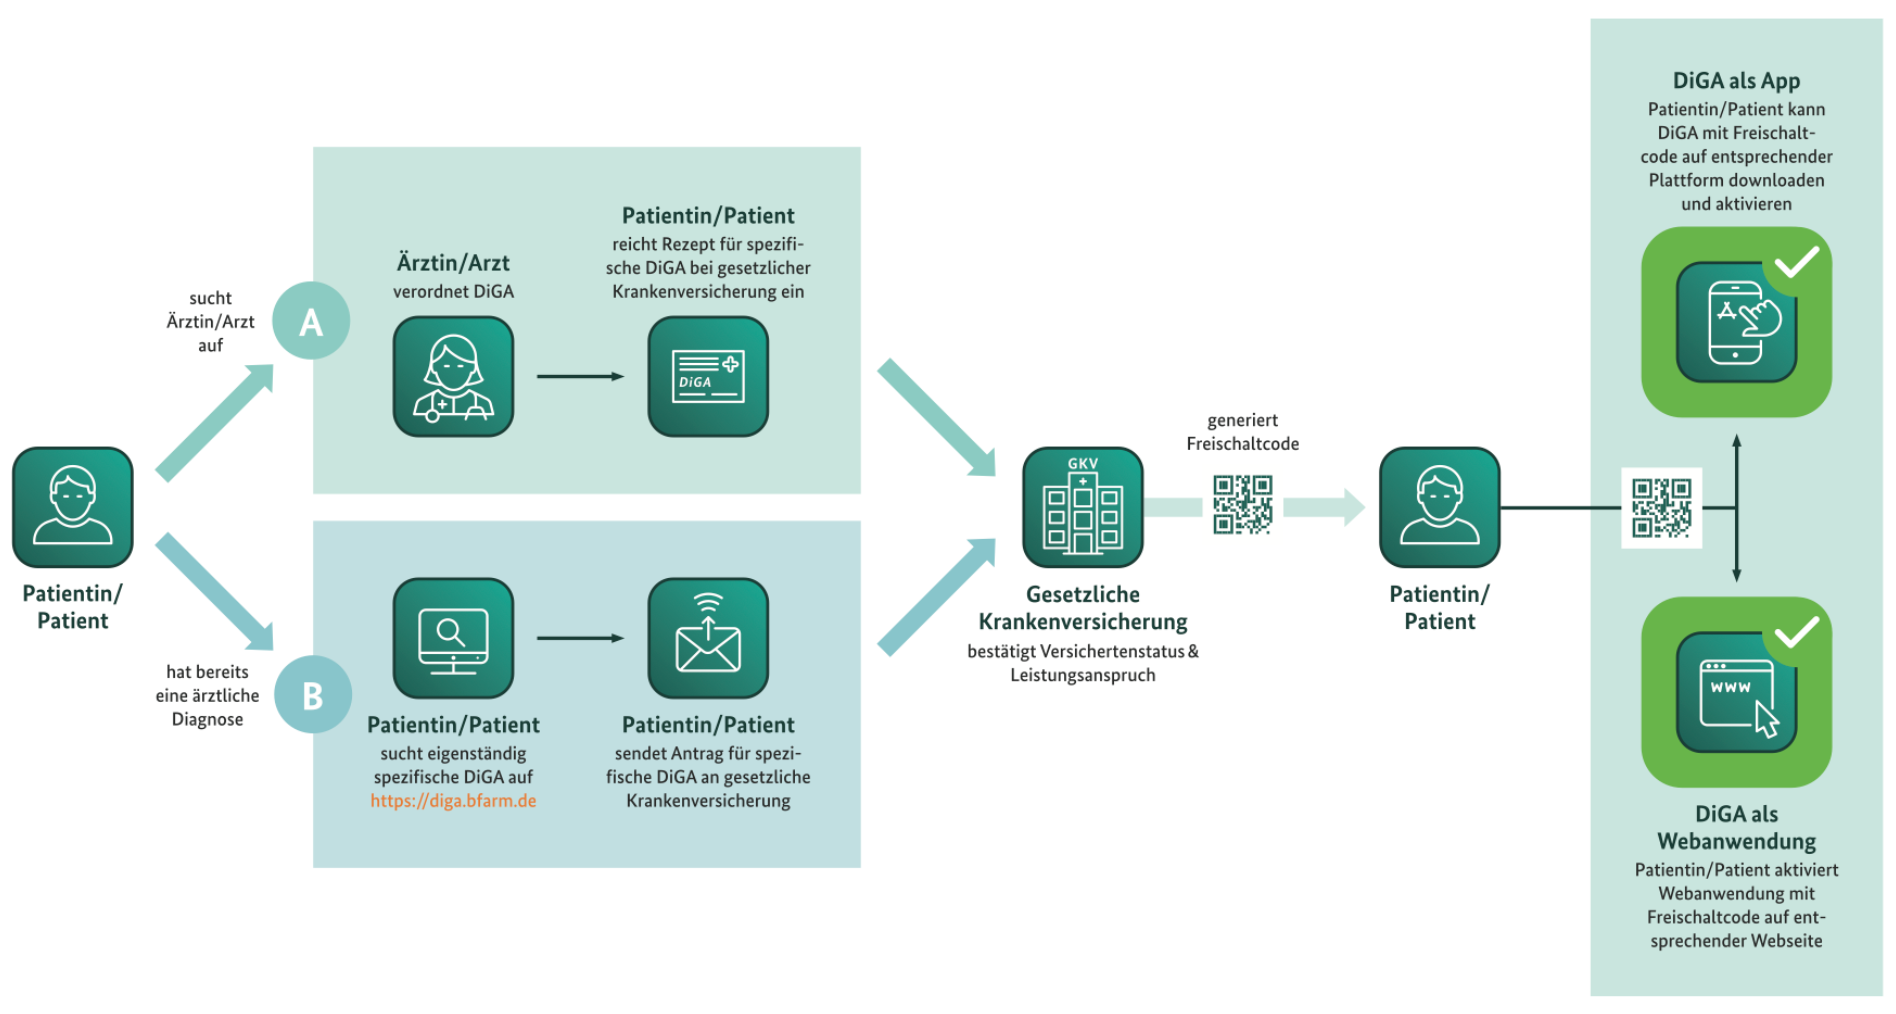
\includegraphics[width=450px, keepaspectratio]{assets/verordnungs_prozess.png}
	\caption{Graphauswertung - Komponentendiagramm,\\Quelle: Eigene Darstellung, Tool: \cite{visual_paradigm}}
\end{figure}






\subsection{Wie funktioniert das Fast-Track- Verfahren?}

(https://diga.bfarm.de/de/diga-hersteller)
Wie bereits oben genannt, muss der Hersteller zur Prüfung durch das BfArM einen Antrag zur Aufnahme einer DiGA in das DiGA-Verzeichnis stellen ,sodass dann das Anliegen und ob dieses den Voraussetzungen entspricht geprüft werden.
Die gestellten Anforderungen an die DiGa beziehen sich auf die Sicherheit , Qualität, Verwendbarkeit, Interoperabilität , Datensicherheit und den Datenschutz.
Was jedoch ebenso von großer Relevanz ist , ist dass die positiven Versorgungseffekte , wie der medizinische Nutzen und die Verfahrens- und Strukturverbesserungen gewährleistet werden können.
Anhand der Prüfung wird entschieden , ob die DiGa direkt abgelehnt, bei halb erkennbarem Genügen in die vorläufige Aufnahme zur weiteren Testung während des Verfahrens geschickt oder direkt bestätigt und eingetragen wird.
Falls die DiGa nur teilweise den Voraussetzungen entspricht , wird sie vorläufig aufgenommen in das DiGa-Verzeichnis , muss jedoch eine ca. 12 Monatige Erprobungsphase durchlaufen.
Nach Abschluss des Verfahrens erhält der Hersteller einen Entscheid, ob seine DiGA die Voraussetzungen zur Aufnahme in das DiGA-Verzeichnis erfüllt. 
In der Abbildung sind die einzelnen Vorkehrungen
des Prozesses dargestellt.

\begin{figure}[H]
	\centering
	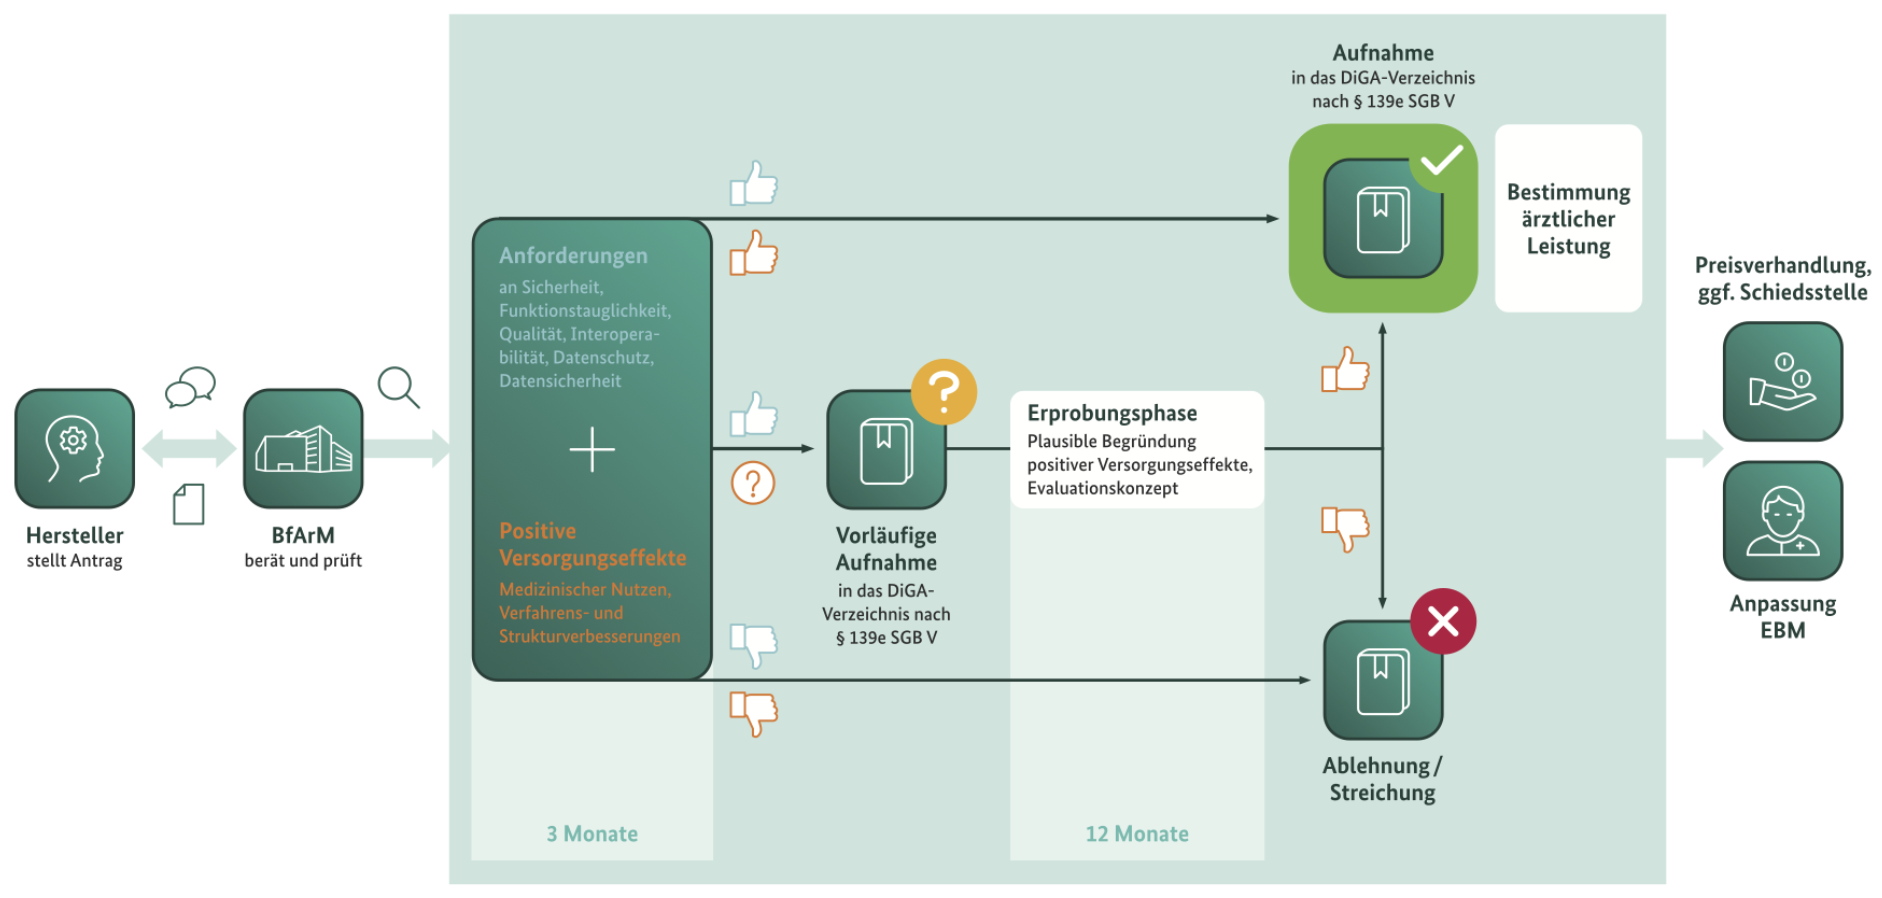
\includegraphics[width=450px, keepaspectratio]{assets/fastTrack_prozess.png}
	\caption{Graphauswertung - Komponentendiagramm,\\Quelle: Eigene Darstellung, Tool: \cite{visual_paradigm}}
\end{figure}
